\documentclass[english]{beamer}
\usetheme{Frankfurt}

\title{Finite temperature and $\delta$-regime in the Schwinger model}
\author{
  Ivan Hip\textsuperscript{a},
  Jaime Fabián Nieto Castellanos\textsuperscript{b},
  Wolfgang Bietenholz\textsuperscript{b}}
\institute{
  \textsuperscript{a}University of Zagreb, Croatia\\
  \textsuperscript{b}UNAM, Mexico
}
\date{July 29, 2021}

\begin{document}
 
\begin{frame}
  \titlepage
\end{frame}

\section{Introduction}

\begin{frame}{Schwinger model}
\end{frame}


\section{Finite temperature}

\begin{frame}{Finite temperature - Hosotani prediction}
  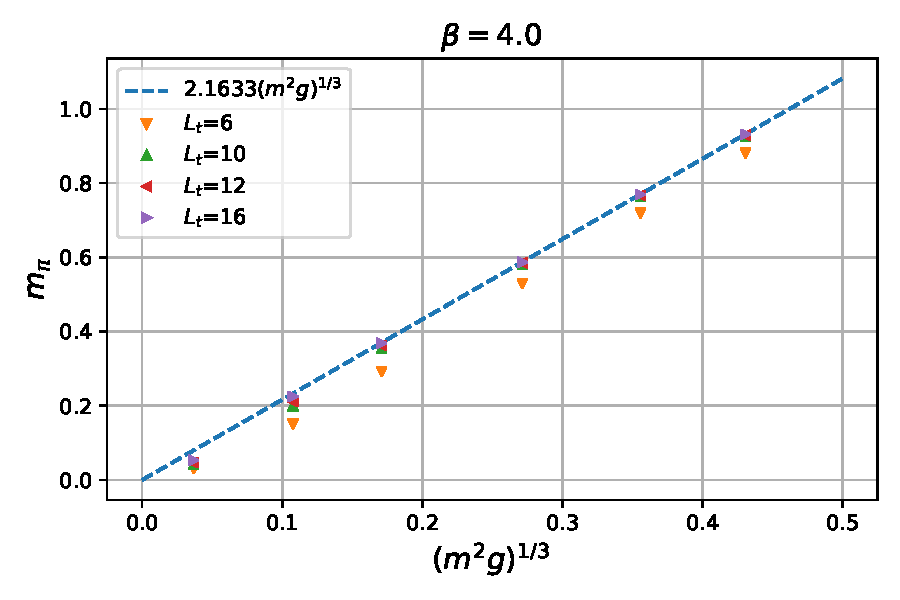
\includegraphics[width=1\textwidth]{figs/FiniteTMPiHos}
\end{frame}

\begin{frame}{Pion mass - Hosotani vs. lattice simulation}
  \includegraphics[width=1\textwidth]{figs/MPi64x10FiniteT}
\end{frame}

\begin{frame}{Pion mass - Hosotani vs. lattice simulation}
  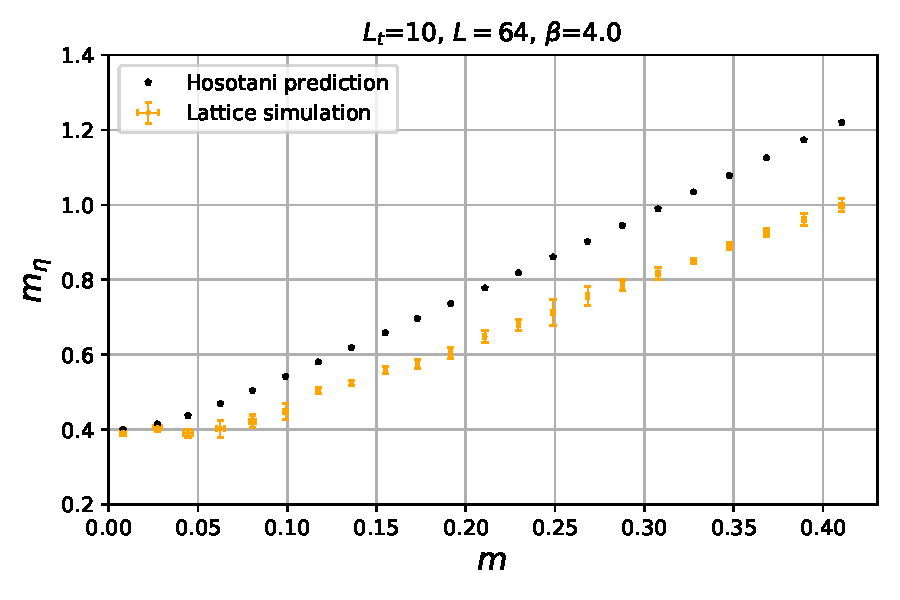
\includegraphics[width=1\textwidth]{figs/Meta64x10FiniteT}
\end{frame}

\section{$\delta$-regime}

\begin{frame}{$\delta$-regime}
\end{frame}

\begin{frame}{Hasenfratz/Niedermayer prediction}
\end{frame}

\begin{frame}{Residual pion mass plateau}
  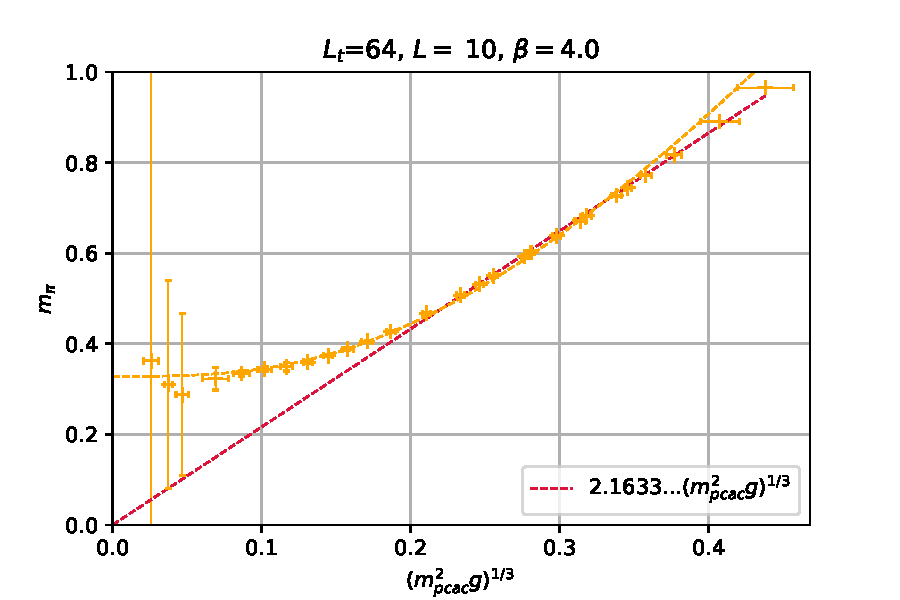
\includegraphics[width=1\textwidth]{figs/Mpi10x64}
\end{frame}

\begin{frame}{Residual pion mass plateau}
  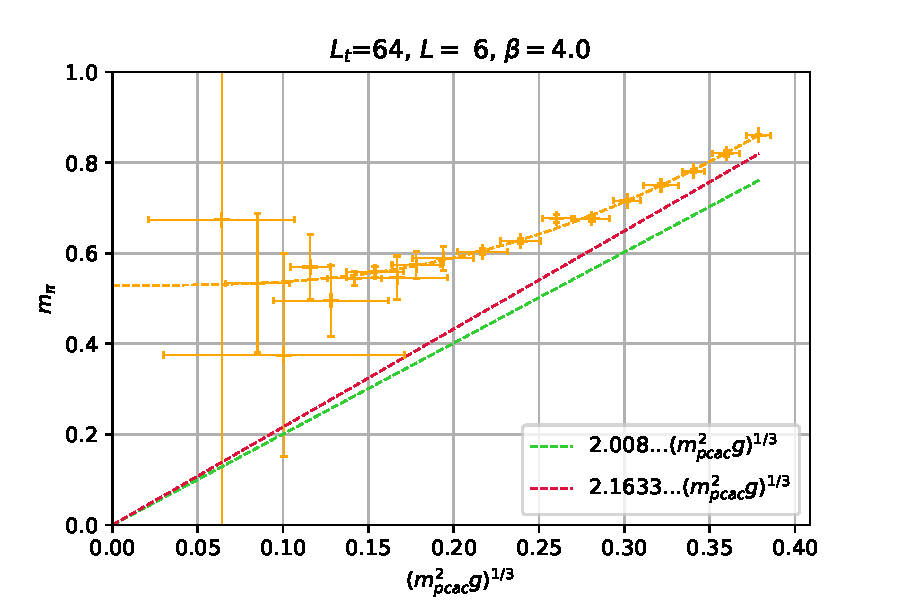
\includegraphics[width=1\textwidth]{figs/Mpi6x64Pt10}
\end{frame}

\begin{frame}{1 / L confirmed by lattice simulation}
  \begin{columns}[t]
    \column{0.5\textwidth}
      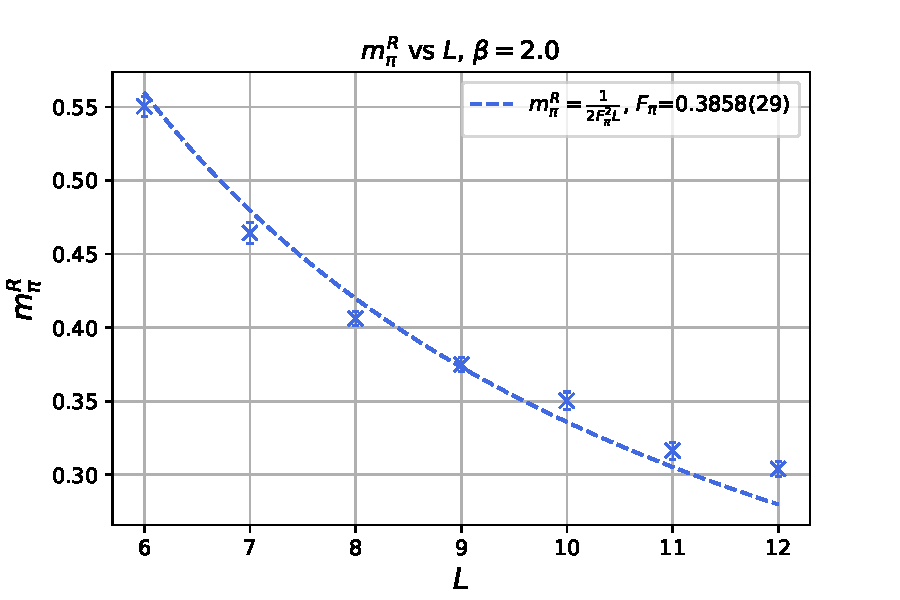
\includegraphics[width=1.0\textwidth]{figs/ResMpiBeta2}
      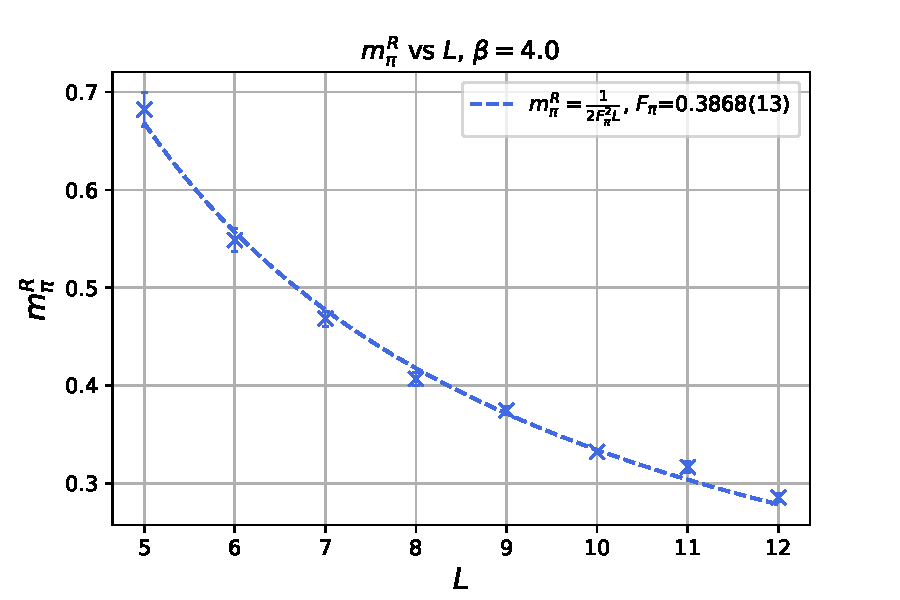
\includegraphics[width=1.0\textwidth]{figs/ResMpiBeta4}
    \column{0.5\textwidth}
      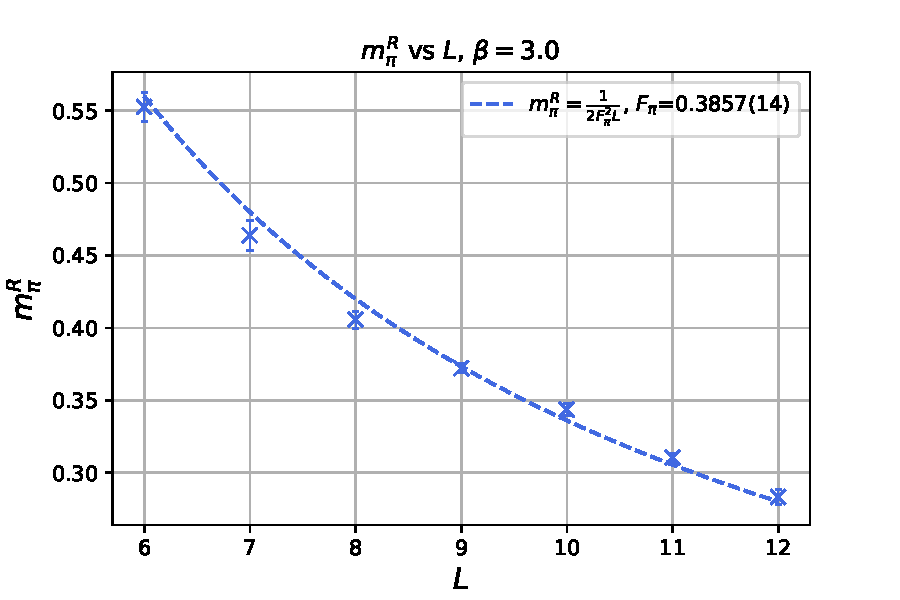
\includegraphics[width=1.0\textwidth]{figs/ResMpiBeta3}
      \[
      	F_\pi = 0.7
      \]
  \end{columns}
\end{frame}


\section{Witten-Veneziano}

\begin{frame}{Witten-Veneziano formula}
In the chiral $N$-flavor Schwinger model the Witten-Veneziano formula is simplified to [Seiler and
Stamatescu, 1987]
\[
  m_\eta^2 = \frac{2N}{F_\eta^2}\chi_T^{que}
\]
Mass of the $\eta$ particle is known analytically [Belvedere et al. 1979] 
\[
  m_\eta^2 = \frac{N}{\pi\beta}
\]
and there is also continuum prediction for $\chi_T^{que}$
[Seiler and Stamatescu, 1987]
\[
  \beta\chi_T^{que} = \frac{1}{4\pi^2}
\]
\end{frame}

\begin{frame}{Quenched topological susceptibility}
By using an alternative definition of topological charge
\[
  Q_S = \frac{1}{2\pi}\sum_{P}\sin(\theta_P)
\]
[Bardeen et al., 1998] were able to analytically compute
$\chi_T^{que}$ on the lattice
\[
  \beta\chi_T^{que} = \frac{I_1(\beta)}{4 \pi^2 I_0(\beta)}
\]
For the usual definition of topological charge
\[
  Q_T = \frac{1}{2\pi}\sum_{P}\theta_P
\]
it is not possible to find analytic solution, but using the 
same line of reasoning it is possible to numerically compute
$\chi_T^{que}$ to arbitrary precision.
\end{frame}

\begin{frame}{Quenched topological susceptibility}
  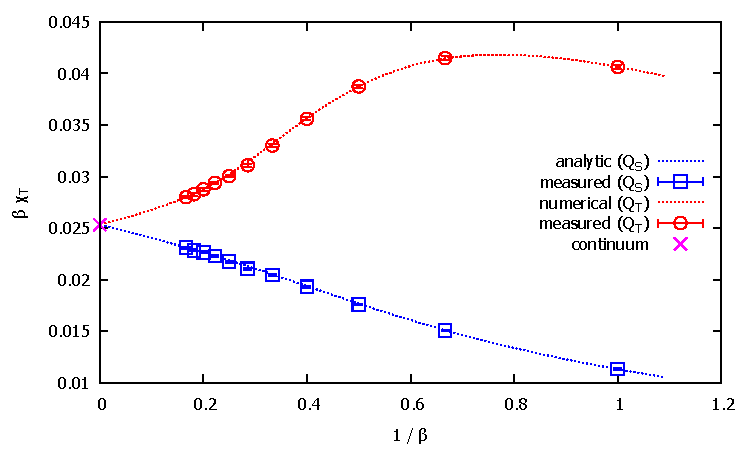
\includegraphics[width=1\textwidth]{figs/BeakDiagram}
\end{frame}

\begin{frame}{$F_\eta$ versus $F_\pi$}
\end{frame}

\end{document}
